Ahora pensemos que una componente de momentum está fija, con valor $p_1$. Los estados compatibles con esta condición forman un anillo, que también es un cascarón esférico, pero en $3 \mathrm{~N}-1$ dimensiones, y de radio $R^{\prime}=\sqrt{2 m E-p_1^2}$.
\begin{figure}[h]
    \centering
    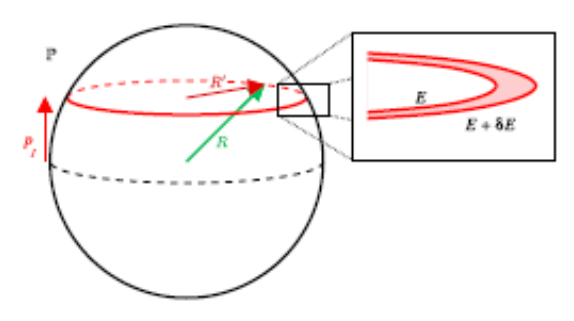
\includegraphics[width=0.5\textwidth]{punto1/cascaron.png}
    \caption{Cascaron esferico en 3 dimensiones}
    \label{fig:f1}
\end{figure}

